\section{支线}

本节旨在介绍一些零散而有用的代数知识.

\subsection{模格}

\begin{definition}[格]
    一个偏序集 \((L,\leq)\) 称一个格 (lattice) 当对任意 \(a,b\in L\) 都有上确界 \(a \vee b\) 和下确界 \(a \wedge b\).

    若有 \(1 := \sup L\) 和 \(0 := \inf L\), 则称 \(L\) 为有界格, 任何格都可以嵌入有界格.
\end{definition}

\begin{corollary}
    格有有限非空集的上界和下界.
\end{corollary}

\begin{definition}[对偶格]
    对 \(L\) 的格 \((L,\leq)\), 定义 \(L^{\text{op}}\) 为 \((L,\geq)\) 的格, 称为 \(L\) 的对偶格.
\end{definition}

\begin{definition}[区间]
    对 \(a \leq b\) 定义 \([a,b] := \{x\in L : a \leq x \leq b\}\) 为 \(a\) 和 \(b\) 定义的区间.
\end{definition}

\begin{remark}
    可定义 \(a \leq b \iff a \vee b = b\), 故格的结构仅由 \((L,\vee,\wedge)\) 完全确定.
\end{remark}

\begin{lemma}
    以下不等式总成立:

    \[
        \begin{aligned}
            (x \wedge y) \vee (x \wedge z) &\leq x \wedge (y \vee z) \\
            x \vee (y \wedge z) &\leq (x \vee y) \wedge (x \vee z) \\
            (x \wedge y) \vee (x \wedge z) \vee (y \wedge z) &\leq (x \vee y) \wedge (x \vee z) \wedge (y \vee z) \\
            (x \wedge y) \vee (x \wedge z) &\leq x \wedge (y \vee (x \wedge z))
        \end{aligned}
    \]

    \begin{proof}
        计算, 如第四条不等式有:

        \[
            \begin{aligned}
                x \wedge y &\leq x \\
                x \wedge z &\leq x \\
                x \wedge y &\leq y \leq y \vee (x \wedge z) \\
                x \wedge z &\leq y \vee (x \wedge z)
            \end{aligned}
        \]
    \end{proof}
\end{lemma}

\begin{definition}[理想]
    \(I \subseteq L\) 称理想若 \(\forall a \in I \forall b \in L (a \wedge b \in I)\).

    素理想则还要求 \((a \vee b \in I) \implies (a \in I) \lor (b \in I)\).
\end{definition}

\begin{definition}[滤子]
    \(F \subseteq L\) 称滤子若 \(\forall a \in F \forall b \in L (a \vee b \in F)\).
\end{definition}

\begin{definition}[凸]
    一个子集 \(C \subseteq L\) 称凸若 \(\forall a,c \in C \forall b \in L (a \leq b \leq c \implies b \in C)\).
\end{definition}

\begin{lemma}
    若理想 \(I\) 与滤子 \(F\) 的交非空, 则其诱导了凸子集 \(I \cap F\), 且所有凸子格都可以由理想与滤子的交得到.

    \begin{proof}
        有 \((a \leq b) \land (b \in I) \implies (a = a \wedge b \in I)\), 以及 \((a \leq b) \land (a \in F) \implies (b = a \vee b \in F)\), 故 \(I \cap F\) 为凸子格.

        反之, 若 \(C\) 为凸子格, 则 \(I := \{a \in L : \exists b \in C (a \leq b)\}\) 为理想, \(F := \{b \in L : \exists a \in C(a \leq b)\}\) 为滤子, 且 \(C = I \cap F\).
    \end{proof}
\end{lemma}

\begin{definition}[模格]
    若 \(c \vee (a \wedge b) = a \wedge (c \vee b)\) 对任意 \(a,b,c,c \leq a\) 都成立, 则称 \(L\) 为模格.
\end{definition}

\begin{definition}
    有界模格中 \(a\) 若有 \(b\) 使得 \(a \vee b = 1, a \wedge b = 0\), 则称 \(b\) 为 \(a\) 补, 记作 \(a^{\bot}\).
\end{definition}

\begin{definition}[Boolean 环]
    \setlabel {Boolean 环}
    \label {definition:boolean ring}
    一个交换幺环 \(R\) 称为 Boolean 环若 \(x^2 = x\) 对任意 \(x \in R\) 都成立, 显然 Boolean 环的子环商环均为 Boolean 环.
\end{definition}

\begin{lemma}
    设 \(R\) 是 Boolean 环, 则:

    \begin{enumerate}
        \item \(\mathrm{char} (R) = 2\)
        \item 素理想 \(\mathfrak{p}\) 均极大, 且 \(R / \mathfrak{p} = \mathbb{F}_2\)
        \item 有限生成理想均为主理想.
    \end{enumerate}

    \begin{proof}
        对于第一条, 有 \(2x = 4x - 2x = 4x^2 - 2x = {(2x)}^2 - 2x = 2x - 2x = 0\),
        对于第二条, 有 \(x (1-x) = x - x^2 = 0\), 故 \(A / \mathfrak{p}\) 至多二元, 且其为整环, 故必为 \(\mathbb{F}_2\),
        对于第三条, 注意到 \(ma + nb = (a + b + ab) (ma + nb)\) 即可.
    \end{proof}
\end{lemma}

\begin{definition}[Boolean 格]
    一个模格 \(L\) 称为 Boolean 格若 \(L\) 为有界模格且所有元素均有补.
\end{definition}

\begin{lemma}
    给出 \(a + b = (a \wedge b^{\bot}) \vee (a^{\bot} \wedge b)\), \(ab = a \wedge b\), 对称的, 给出
    \(a \vee b = a + b + ab\), \(a \wedge b = ab\), \(a \leq b \iff a = ab\) 给出了 Boolean 格与 Boolean 环的一一对应.
\end{lemma}

\begin{lemma}
    给出格 \(L\), 其为模格当且仅当对于区间 \(I\), \(a\) 有两个补 \(c_1,c_2\), 则 \(c_1 \leq c_2 \implies c_1 = c_2\).

    \begin{proof}
        \(\implies\) : 给出区间 \([n,m]\), 有 
        
        \[
            c_1 = c_1 \wedge m = c_1 \wedge (a \vee c_2) = (c_1 \wedge a) \vee c_2 = n \wedge c_2 = c_2
        \]

        \(\impliedby\) : 若给出 \(a \leq A\), 注意到 \(a \vee (A \wedge b),A \wedge (a \vee b)\) 均为 \([A \wedge b,a \vee b]\) 中 \(b\) 的补.
    \end{proof}
\end{lemma}

\begin{definition}[格图]
    我们用线表示偏序关系, 从高到底由大到小, 称为格图 (lattice diagram).
\end{definition}

\begin{lemma}
    模格中有标准同构 \([a \wedge b,a] \to [b,a \vee b]\).

    \begin{proof}
        直接构造双射 \(x \mapsto x \vee b\), \(x \mapsto x \wedge a\).
    \end{proof}
\end{lemma}

\begin{lemma}[Zassenhaus 引理]
    \setlabel {Zassenhaus 引理}
    \label {lemma:Zassenhaus lemma}
    令 \(u \leq U,v \leq V\) 则有格图如下:

    \begin{center}
        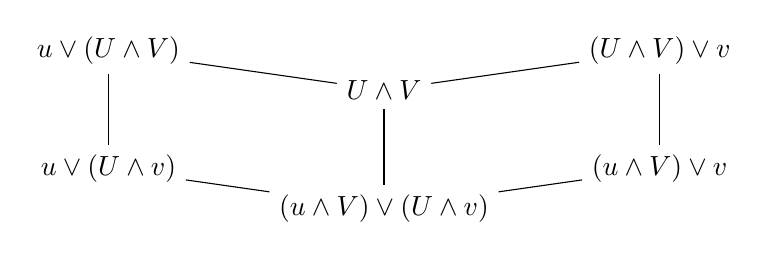
\begin{tikzpicture}
            \node (uUV) at (-3.5,1) {\(u \vee (U \wedge V)\)};
            \node (UVv) at (3.5,1) {\((U \wedge V) \vee v\)};
            \node (UV) at (0,.5) {\(U \wedge V\)};
            \node (uUv) at (-3.5,-.5) {\(u \vee (U \wedge v)\)};
            \node (uVv) at (3.5,-.5) {\((u \wedge V) \vee v\)};
            \node (uVUv) at (0,-1) {\((u \wedge V) \vee (U \wedge v)\)};

            \draw (uUV) to (UV); \draw (UVv) to (UV);
            \draw (uUv) to (uVUv); \draw (uVv) to (uVUv);
            \draw (uUV) to (uUv); \draw (UVv) to (uVv); \draw (UV) to (uVUv);
        \end{tikzpicture}
    \end{center}

    上述格图给出同构:

    \[
        [u \vee (U \wedge v), u \vee (U \wedge V)] \to [(u \wedge V) \vee v, (U \wedge V) \vee v]
    \]

    \begin{proof}
        我们证明其均同构于 \([(u \wedge V) \vee (U \wedge v),U \wedge V]\), 由于格图对称, 只需证明左半部分, 令 \(b = u \vee (U \wedge v), a = U \wedge V\), 
        则 \(a \vee b = (U \wedge V) \vee u \vee (U \wedge v) = u \vee (U \wedge V)\), \(a \wedge b = (U \wedge V) \wedge (u \vee (U \wedge v)) = (U \wedge v) \vee (U \wedge V \wedge u) = (u \wedge V) \vee (U \wedge v)\).
    \end{proof}
\end{lemma}

\begin{definition}
    模格中的两条降链 \(x_0 \geq x_1 \geq \cdots \geq x_n\) 和 \(y_0 \geq y_1 \geq \cdots \geq y_n\) 称等价若存在 \(\sigma \in S_{n}\) 使得 \([x_{i+1},x_i] \cong [y_{\sigma (i) + 1},y_{\sigma (i)}]\).
\end{definition}

\begin{theorem}[Schreier 加细定理]
    \setlabel {Schreier 加细定理}
    \label {theorem:Schreier refinement theorem}
    给出降链 \(x_0 \geq x_1 \geq \cdots \geq x_m\) 和 \(y_0 \geq y_1 \geq \cdots \geq y_n\), 满足 \(x_0 = y_0 \land x_m = y_n\),
    则存在加细 \(x_0 = z_0 \geq z_1 \geq \cdots \geq z_k = x_m\) 和 \(y_0 = w_0 \geq w_1 \geq \cdots \geq w_k = y_n\) 使得 \(z\) 和 \(w\) 等价.

    \begin{proof}
        令 \(x_{i,j} = x_{i+1} \vee (x_i \wedge y_j)\), \(y_{i,j} = y_{i+1} \vee (y_i \wedge x_j)\), 利用 \ref{lemma:Zassenhaus lemma} 给出
        \([x_{i,j+1},x_{i,j}] \cong [y_{j,i+1},y_{j,i}]\).
    \end{proof}
\end{theorem}

\begin{definition}[合成列]
    \(a < b\) 的合成列 (composition series) 是指一个极长降列 \(a = x_0 > x_1 > \cdots > x_n = b\).
\end{definition}

\begin{theorem}[Jordan-Hölder 定理]
    \setlabel {Jordan-Hölder 定理}
    \label {theorem:Jordan-Holder theorem}
    任意两个合成列等价.

    \begin{proof}
        利用 \ref{theorem:Schreier refinement theorem} 给出加细.
    \end{proof}
\end{theorem}

\begin{definition}[有限长度]
    一个模格称 Noether 若其满足 \ref{definition:ascending chain condition}, Artin 若其满足 \ref{definition:descending chain condition}.

    既 Noether 又 Artin 的模格称为有限长度的.
\end{definition}

\begin{lemma}
    给定 \(a < b\), \([a,b]\) 有限长度当且仅当 \(a,b\) 有合成列.

    \begin{proof}
        假定给出无穷升列或降列, 添入 \([a,b]\) 构造出任意长度的非平凡列, 故合成列长度的下限发散.

        反之, 对于有限长度的 \([a,b]\), 令 \(x_0 = b\) 依赖 Noether 性质寻找极大 \(x_{i+1} \in [a,x_i] \setminus \{x_i\}\), 依 Artin 性质知其止于 \(a\).
    \end{proof}
\end{lemma}

\begin{corollary}
    对于有限长度 \(L\), 任意 \(a,b\) 间的列可加细为合成列.
\end{corollary}

\begin{definition}[长度]
    \setlabel {长度}
    \label {definition:length of a module lattice}
    取有限长度的有界模格 \(L\), 若合成列满足 \(x_0 = 1\), \(x_n = 0\), 则称 \(n\) 为其长度.
\end{definition}

